
Writing unit tests is technically possible without any kind of framework. All we have to do is create an instance of the class we want to test, execute one of its methods, and check if the new state or value returned meets our expectations. Then, we report the result and delete the object under test. Let's try it out.

We'll use the following structure:

\begin{tcblisting}{commandshell={}}
- CMakeLists.txt
- src
     |- CMakeLists.txt
     |- calc.cpp
     |- calc.h
     |- main.cpp
- test
     |- CMakeLists.txt
     |- calc_test.cpp
\end{tcblisting}

Starting from main.cpp, we can see it will use a Calc class, as illustrated in the following code snippet:

\begin{lstlisting}[style=styleCXX]
// chapter08/01-no-framework/src/main.cpp

#include <iostream>
#include "calc.h"
using namespace std;

int main() {
	Calc c;
	cout << "2 + 2 = " << c.Sum(2, 2) << endl;
	cout << "3 * 3 = " << c.Multiply(3, 3) << endl;
}
\end{lstlisting} 

Nothing too fancy—main.cpp simply includes the calc.h header and calls two methods of the Calc object. Let's quickly glance at the interface of Calc, our SUT, as follows:

\begin{lstlisting}[style=styleCXX]
// chapter08/01-no-framework/src/calc.h

#pragma once
class Calc {
	public:
	int Sum(int a, int b);
	int Multiply(int a, int b);
};
\end{lstlisting} 

The interface is as simple as possible. We're using \#pragma once here—it works exactly like commonly seen preprocessor include guards and is understood by almost all modern compilers, despite not being part of the official standard. Let's see the class implementation, as follows:

\begin{lstlisting}[style=styleCXX]
// chapter08/01-no-framework/src/calc.cpp

#include "calc.h"
int Calc::Sum(int a, int b) {
	return a + b;
}

int Calc::Multiply(int a, int b) {
	return a * a; // a mistake!
}
\end{lstlisting} 

Uh-oh! We introduced a mistake! Multiply is ignoring the b argument and returns a squared instead. That should be detected by correctly written unit tests. So, let's write some! Here we go:

\begin{lstlisting}[style=styleCXX]
// chapter08/01-no-framework/test/calc_test.cpp

#include "calc.h"
#include <cstdlib>

void SumAddsTwoIntegers() {
	Calc sut;
	if (4 != sut.Sum(2, 2))
	std::exit(1);
}

void MultiplyMultipliesTwoIntegers() {
	Calc sut;
	if(3 != sut.Multiply(1, 3))
	std::exit(1);
}
\end{lstlisting} 

We start our calc\_test.cpp file by writing two test methods, one for each tested method of SUT. If the value returned from the called method doesn't match expectations, each function will call std::exit(1). We could use assert(), abort(), or terminate() here, but that would result in a less explicit Subprocess aborted message in the output of ctest, instead of the more readable Failed message.

Time to create a test runner. Ours will be simple as possible because doing it correctly would require a ridiculous amount of work. Just look at the main() function we had to write in order to run just two tests:

\begin{lstlisting}[style=styleCXX]
chapter08/01-no-framework/test/unit_tests.cpp
#include <string>
void SumAddsTwoIntegers();

void MultiplyMultipliesTwoIntegers();

int main(int argc, char *argv[]) {
	if (argc < 2 || argv[1] == std::string("1"))
		SumAddsTwoIntegers();
	
	if (argc < 2 || argv[1] == std::string("2"))
		MultiplyMultipliesTwoIntegers();
}
\end{lstlisting} 

Here's a breakdown of what happens here:

\begin{itemize}
\item 
We declare two external functions that will be linked from another translation unit.

\item 
If no arguments were provided, execute both tests (the zeroth element in argv[] is always the program name).

\item 
If the first argument is an identifier of the test, execute it.

\item 
If any of the tests fail, it internally calls exit() and returns with a 1 exit code.

\item 
If no tests were executed or all passed, it implicitly returns with a 0 exit code.
\end{itemize}

To run the first test, we'll execute ./unit\_tests 1; to run the second, we'll execute ./unit\_tests 2. We simplified the code as much as we could, and it still turned out to be pretty hard to read. Anyone who might need to maintain this section isn't going to have a great time after adding a few more tests, not to mention that this functionality is pretty raw—debugging such a test suite will be a lot of work. Nevertheless, let's see how we can use it with CTest, as follows:

\begin{lstlisting}[style=styleCMake]
# chapter08/01-no-framework/CMakeLists.txt


cmake_minimum_required(VERSION 3.20.0)
project(NoFrameworkTests CXX)
enable_testing()
add_subdirectory(src bin)
add_subdirectory(test)
\end{lstlisting} 

We start with the usual heading and enable\_testing(). This is to tell CTest that we'd like to enable tests in this directory and its subdirectories. Next, we'll include two nested listfiles in each of the subdirectories: src and test. The highlighted bin value states that we'd like the binary output of src subdirectories to be placed in <build\_tree>/ bin. Otherwise, binary files would end up in <build\_tree>/src, which could be confusing. After all, build artifacts are no longer source files.

The listfile for the src directory is very straightforward and contains a simple main target definition, as illustrated here:

\begin{lstlisting}[style=styleCMake]
# chapter08/01-no-framework/src/CMakeLists.txt

add_executable(main main.cpp calc.cpp)
\end{lstlisting} 

We also need a listfile for the test directory, as follows:

\begin{lstlisting}[style=styleCMake]
# chapter08/01-no-framework/test/CMakeLists.txt

add_executable(unit_tests
				unit_tests.cpp
				calc_test.cpp
				../src/calc.cpp)
target_include_directories(unit_tests PRIVATE ../src)

add_test(NAME SumAddsTwoInts COMMAND unit_tests 1)
add_test(NAME MultiplyMultipliesTwoInts COMMAND unit_tests 2)
\end{lstlisting} 

We have now defined a second unit\_tests target that also uses the src/calc. cpp implementation file and respective header. Finally, we explicitly add two tests: SumAddsTwoInts and MultiplyMultipliesTwoInts. Each provides its ID as an argument to the add\_test() command. CTest will simply take anything provided after the COMMAND keyword and execute it in a subshell, collecting the output and exit code. Don't get too attached to add\_test()—in the Unit-testing frameworks section, we'll discover a much better way of dealing with test cases, so we'll skip describing it in detail here.

This is how ctest works in practice when executed in the build tree:

\begin{tcblisting}{commandshell={}}
# ctest
Test project /tmp/b
       Start 1: SumAddsTwoInts
1/2 Test #1: SumAddsTwoInts ................... Passed
0.00 sec
       Start 2: MultiplyMultipliesTwoInts
2/2 Test #2: MultiplyMultipliesTwoInts ........***Failed
0.00 sec

50% tests passed, 1 tests failed out of 2
Total Test time (real) = 0.00 sec
The following tests FAILED:
             2 - MultiplyMultipliesTwoInts (Failed)
Errors while running CTest
Output from these tests are in: /tmp/b/Testing/Temporary/
LastTest.log
Use "--rerun-failed --output-on-failure" to re-run the failed
cases verbosely.
\end{tcblisting}

CTest executed both tests and reported that one of them is failing—the returned value from Calc::Multiply didn't meet expectations. Very good. We now know that our code has a bug, and someone should fix it.

\begin{tcolorbox}[colback=blue!5!white,colframe=blue!75!black,title=Note]
You may have noticed that in most examples so far, we didn't necessarily employ the project structure described in Chapter 3, Setting Up Your First CMake Project. This was done to keep things brief. This chapter discusses more advanced concepts, and therefore using a full structure is warranted. In your projects (no matter how small), it's best to follow this structure from the start. As a wise man once said: "You step onto the road, and if you don't keep your feet, there's no knowing where you might be swept off to."
\end{tcolorbox}

It's no secret that you should avoid building a testing framework as part of your own project. Even the most basic example is hard on the eyes, has a lot of overhead, and doesn't add any value. However, before we can adopt a unit-testing framework, we'll need to rethink the structure of the project.

\subsubsubsection{8.4.1\hspace{0.2cm}Structuring our projects for testing}

C++ has some limited introspection capabilities, but cannot offer such powerful retrospection features as Java can. This might be the very reason why writing tests and unit-testing frameworks for C++ code is much harder than in other, richer environments. One implication of such an economic approach is the fact that the programmer has to be more involved in crafting testable code. We'll not only have to design our interfaces more carefully, but also answer questions about the practicalities, such as this: How do we avoid doubling the compilation, and reuse artifacts between tests and production?

Compilation time might not be a significant problem for smaller projects, but as time flies, the projects grow. The need for short compilation loops does not go away. In the previous example, we appended all the sut sources to the unit-test executable apart from the main.cpp file. If you were reading closely, you will have noticed that we had some code in that file that didn't get tested (the contents of main() itself). By compiling the code twice, there's a slight chance that the produced artifacts won't be exactly the same. These things can potentially diverge over time (due to the addition of compilation flags and preprocessor directives). This may be especially dangerous when engineers contributing to the code base are in a rush, inexperienced, or simply unfamiliar with the project.

There are multiple ways of dealing with the problem, but the most elegant is to build your entire solution as a library and link it with unit tests. You might ask: "How are we going to run it then?" We'll need a bootstrap executable that will link with the library and run its code.

Begin by renaming your current main() function to run(), start\_program(), or something similar. Then, create another implementation file (bootstrap.cpp) with a new main() function, and this function only. This will be our adapter (or wrapper, if you will): its sole role is to provide an entry point and call the run() forwarding commandline arguments (if any). All that's left is to link everything together, and we've got ourselves a testable project.

By renaming main(), we can now link SUT with tests and test its primary function too. Otherwise, we'd be in violation of the One Definition Rule (ODR) discussed in Chapter 6, Linking with CMake, as the test runner needs its own entry point, a separate main() function. As promised in the Separating main() for testing section of Chapter 6, we'll explain this subject in detail.

The testing framework may provide its own implementation of the main() function out of the box, so we don't need to write it. Usually, it will detect all tests that we've linked and execute them according to the desired configuration.

Artifacts produced by this approach can be grouped into the following targets:

\begin{itemize}
\item 
A sut library with production code

\item 
bootstrap with a main() wrapper calling run() from sut

\item 
unit tests with a main() wrapper that runs all the tests on sut
\end{itemize}

The following diagram shows the symbol relations between targets:

\begin{center}
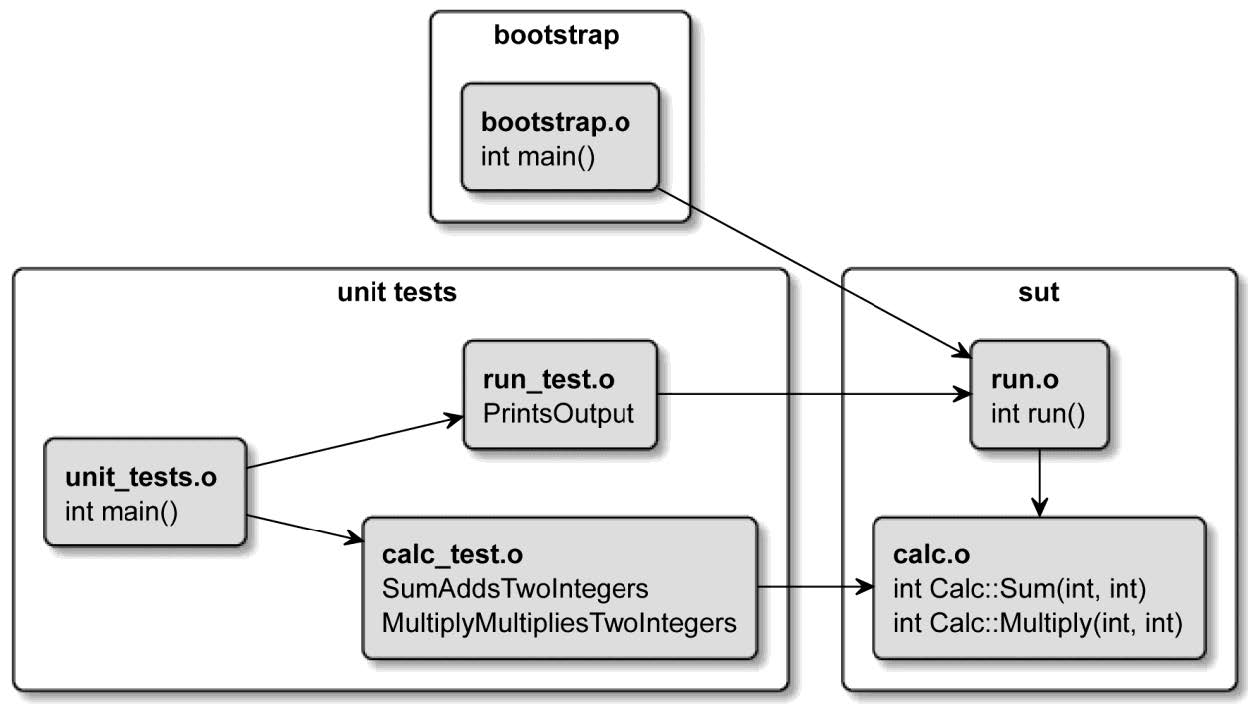
\includegraphics[width=0.8\textwidth]{content/3/chapter8/images/2.jpg}\\
Figure 8.2 ‒ Sharing artifacts between test and production executables
\end{center}

We end up with six implementation files that will produce their respective (.o) object files, as follows:

\begin{itemize}
\item 
calc.cpp—The Calc class to be unit-tested. This is called a unit under test (UUT) because UUT is a specialization of SUT.

\item 
run.cpp—Original entry point renamed run(), which can be now tested.

\item 
bootstrap.cpp—New main() entry point calling run().

\item 
calc\_test.cpp—Tests the Calc class.

\item 
run\_test.cpp—New tests for run() can go here.

\item 
unit\_tests.o—Entry point for unit tests, extended to call tests for run().
\end{itemize}

The library that we're about to build doesn't actually need to be a factual library: static or shared. By creating an object library, we can avoid unnecessary archiving or linking. Technically speaking, it's possible to shave a few moments by relying on dynamic linking for SUT, but more often than not, we're making changes in both targets: tests and sut, canceling out any potential gains.

Let's see how our files have changed, starting with the file previously named main.cpp, as follows:

\begin{lstlisting}[style=styleCXX]
// chapter08/02-structured/src/run.cpp

#include <iostream>
#include "calc.h"
using namespace std;

int run() {
	Calc c;
	cout << "2 + 2 = " << c.Sum(2, 2) << endl;
	cout << "3 * 3 = " << c.Multiply(3, 3) << endl;
	return 0;
}
\end{lstlisting} 

Not too many differences: renamed file and function. We also added a return statement as the compiler won't do this implicitly for functions that are not main().

The new main() function looks like this:

\begin{lstlisting}[style=styleCXX]
// chapter08/02-structured/src/bootstrap.cpp

int run(); // declaration
int main() {
	run();
}
\end{lstlisting} 

As simple as possible—we're declaring that the linker will provide the run() function from another translation unit, and we're calling it. Next to change is the src listfile, which you can see here:

\begin{lstlisting}[style=styleCMake]
# chapter08/02-structured/src/CMakeLists.txt

add_library(sut STATIC calc.cpp run.cpp)
target_include_directories(sut PUBLIC .)

add_executable(bootstrap bootstrap.cpp)
target_link_libraries(bootstrap PRIVATE sut)
\end{lstlisting} 

First, we created a sut library and marked . as a PUBLIC include directory so that it will be propagated to all targets that will link sut (that is, bootstrap and unit\_tests). Note that include directories are relative to the listfile, therefore we can use a dot (.) to refer to the current <source\_tree>/src directory.

Time to update our unit\_tests target. Here, we'll remove the direct reference to the ../src/calc.cpp file with a linking reference to sut for the unit\_tests target. We'll also add a new test for the primary function in the run\_test.cpp file. We'll skip discussing that for brevity, but if you're interested, check out the online examples. Meanwhile, here's the whole test listfile:

\begin{lstlisting}[style=styleCMake]
# chapter08/02-structured/test/CMakeLists.txt

add_executable(unit_tests
				unit_tests.cpp
				calc_test.cpp
				run_test.cpp)
target_link_libraries(unit_tests PRIVATE sut)
\end{lstlisting} 

We should also register the new test, as follows:

\begin{lstlisting}[style=styleCMake]
add_test(NAME SumAddsTwoInts COMMAND unit_tests 1)
add_test(NAME MultiplyMultipliesTwoInts COMMAND unit_tests 2)
add_test(NAME RunOutputsCorrectEquations COMMAND unit_tests 3)
\end{lstlisting} 

Done! By following this practice, you can be sure that your tests are executed on the very machine code that will be used in production.

\begin{tcolorbox}[colback=blue!5!white,colframe=blue!75!black,title=Note]
The target names we're using here, sut and bootstrap, are chosen to make it very clear what they're about from the perspective of testing. In real-life projects, you should pick names that match the context of the production code (rather than tests). For example, for a FooApp, name your target foo instead of bootstrap, and lib\_foo instead of sut.
\end{tcolorbox}

Now that we know how to structure a testable project in appropriate targets, let's shift our focus to the testing frameworks themselves. We don't want to add every test case to our listfiles manually, do we?
































